\documentclass[a4paper]{report}

\usepackage{amsmath}
\usepackage{graphicx}
\usepackage[T1,T2A]{fontenc}
\usepackage[english, russian]{babel}
\usepackage[a4paper, left=2cm, right=2cm, top=2cm, bottom=2cm]{geometry}



\begin{document}
\selectlanguage{russian}
\setlength{\parskip}{6pt}

\noindent
\begin{center}
    \textbf{Билет 1}\\
    Определение определённого интеграла.\\
\end{center}

\textbf{Определение.} Пусть функция $ f(x) $ задана в некотором промежутке $ [a, b] $.
Разобьем этот промежуток произвольным образом на части, вставив между $ a $ и $ b $
точки деления $ (1) $. \emph{Наибольшую} из разностей
$ \Delta x_i = x_{i + 1} - x_{i},\ (i = 0, 1, \ldots, n - 1) $ будем впредь
обозначать через $ \lambda $.

Возьмем в каждом из частичных промежутков $ [x_i, x_{i + 1}] $ по произволу точку 
$ x = \xi_i $. (ранее всегда брали $ \xi_i $ как наименьшее значение $ x_i $).

\begin{center}
    $ x_i \leq \xi_i \leq x_{i + 1},\ (i = 0, 1, \ldots, n - 1) $\\
    и составим сумму $ \sigma = \sum\limits_{i = 0}^{n - 1} f(\xi_i) \Delta x_i $.
\end{center}

\begin{center}
    Установим теперь понятие (конечного) предела этой суммы:\\ 
    \begin{equation}\label{eq3}
        \begin{gathered}
            I = \lim\limits_{\lambda \to 0}{\sigma}
        \end{gathered}
    \end{equation}
\end{center}
Представим себе, что промежуток $ [a, b] $ последовательно разбивается на части,
сначала одним способом, затем -- вторым, третьим и т. д.

\noindent Такую последовательность разбиений промежутка на части мы будем называть 
\emph{основной}, если соответствующая последовательность значений 
$ \lambda = \lambda_1, \lambda_2, \ldots $ сходится к нулю.

Равенство (3) мы понимаем в том смысле, что последовательность значений суммы
$ \sigma $, отвечающая любой \emph{основной} последовательности разбиений промежутка,
всегда стремится к пределу $ I $ как бы не выбирать при этом $ \xi_i $.

Можно и здесь дать определение предела "на языке $ \epsilon $-$ \delta $". Именно,
говорят, что сумма $ \sigma $ при $ \lambda \to 0 $ имеет предел $ I $, если для
каждого числа $ \epsilon > 0 $ найдется такое $ \delta > 0 $, что, лишь только
$ \lambda < \delta $ (т. е. основной промежуток разбит на части, с длинами 
$ \Delta x_i < \delta $), неравенство 

$ |\sigma - I| < \epsilon $

\noindent выполняется при любом выборе чисел $ \xi $.

Конечный предел $ I $ суммы $ \sigma $ при $ \lambda \to 0 $ называется
определённым интегралом функции $ f(x) $ в промежутке от $ a $ до $ b $ и обозначается
\begin{center}
    \begin{equation}\label{eq4}
        \begin{gathered}
            I = \int\limits_{a}^{b} f(x)\ dx\ \text{(обозначение Фурье).}
        \end{gathered}
    \end{equation}
\end{center}
\noindent если такой предел существует, то функция $ f(x) $ называется интегрируемой
на промежутке $ [a, b] $ (где a -- нижний, b -- верхний предел).

Приведенное определение принадлежит Риману, принято называть $ \sigma $ -- римановской
суммой, однако её ещё до Римана использовал Коши, поэтому будем называть её интегральной
суммой.

\noindent \textbf{Notice:} оперделение может быть использовано только для ограниченой функции.
В самом деле если бы функция $ f(x) $ была бы неограничена на $ [a, b] $, то
-- при любом разбиении промежутка на части она бы сохранила подобное свойство
хотя бы в одной из частей. Тогда засчет выбора в этой части точки $ \xi $
можно было бы сделать $ f(\xi) $, а с ней и сумму $ \sigma $ сколь угодно большой;
при этих условиях конечного предела для $ \sigma $, очевидно, существовать не могло бы.
Итак, интегрируемая функция необходимо ограничена.

Поэтому в дальнейшем исследовании мы будем наперед предпологать рассматриваемую функцию
f(x) ограниченной: $ m \leq f(x) \leq M $, if $ a \leq x \leq b $.

\newpage
\textbf{Notice:} Про точки деления (1).
\begin{figure}[ht!]
    \centering
    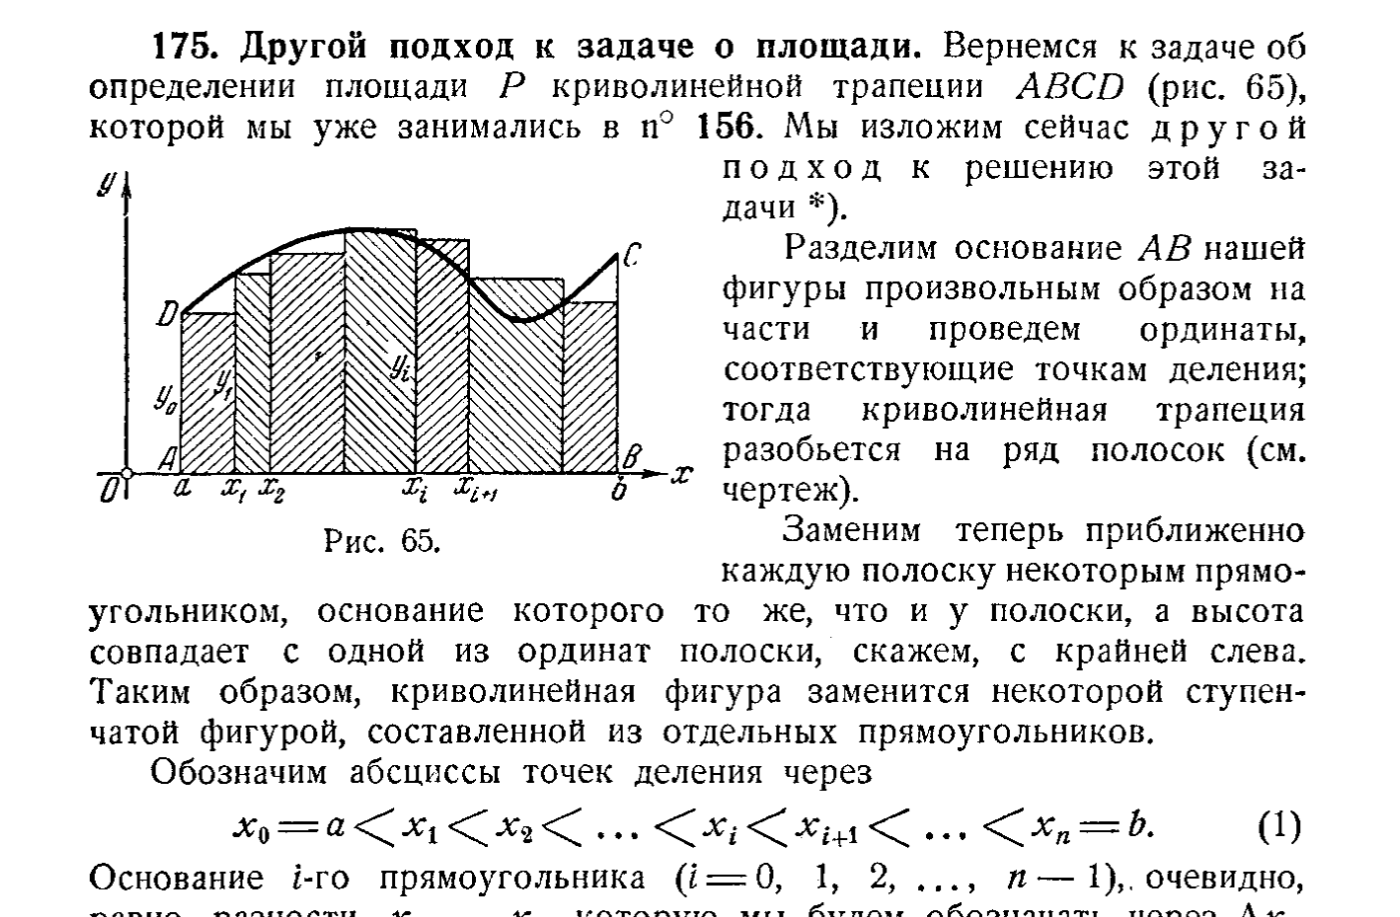
\includegraphics[width=140mm]{int0.png}
\end{figure}

\end{document}
